\section{Acerca de la tesis de licenciatura}




En el trabajo de tesis de licenciatura se analizaron los efectos de las variaciones de los parámetros del clima sobre el desarrollo en la atmósfera de las lluvias atmósferas. Se analizaron datos del arreglo de detectores espaciados 1500 m entre sí, conocido como \emph{arreglo principal}, del Observatorio Pierre Auger, en el periodo 2005-2015 y 2005-2018 extendiendo los periodos de tiempo estudiados anteriormente. Se emuló los resultados de la corrección de la modulación del clima sobre el periodo 2005-2015 de la colaboración Pierre Auger, obteniéndose resultados compatibles. Se observó que posterior a la corrección, la modulación del clima se vio disminuida. Para eventos con energía mayor a $2\,$EeV, esta modulación es despreciable.
  \begin{figure}[H]
    \centering
    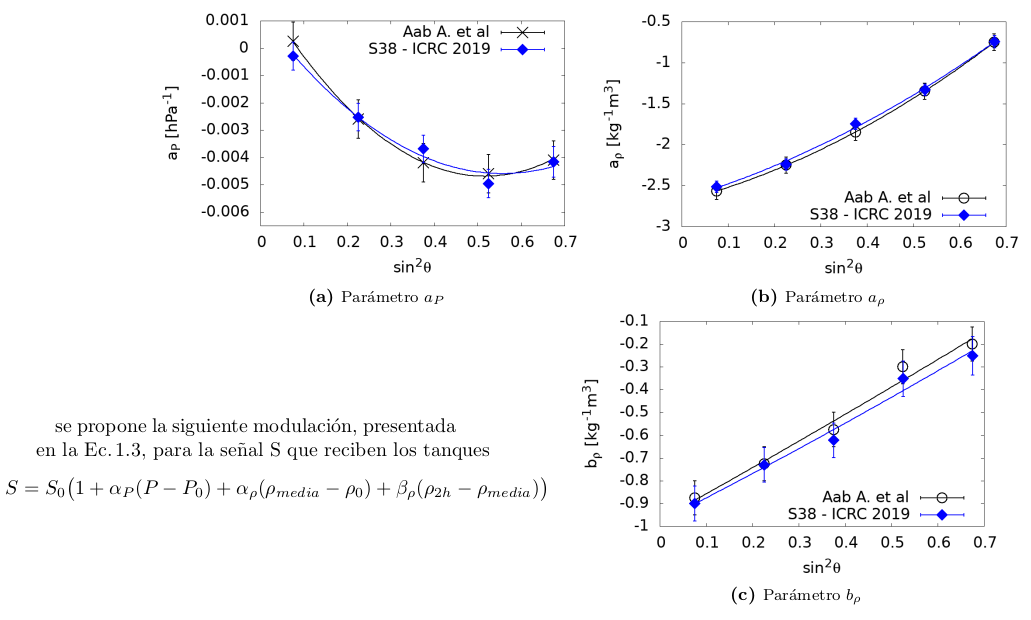
\includegraphics[width=0.95\textwidth]{../beamer-07-05-2020/tesis.png}
  \end{figure}
En el mismo trabajo, se estudió la modulación del clima mediante el valor del $S_{38}$ sin la corrección propuesta por trabajos anteriores. Se observó que los parámetros del clima obtenidos de estos datos son compatibles con los utilizados en la reconstrucción oficial. Se realizó un corrección a  la energía mediante los coeficientes nuevos, observándose que la modulación era despreciable para energías mayores a $2\,$EeV. 

\section{Acerca del archivo con todos los disparos}

La tesis de licenciatura fue realizado sobre los eventos medidos por el arreglo principal utilizando el disparo estándar. Este disparo tiene una eficiencia completa para eventos de energía mayor a $2.5\,$EeV. Por lo que el análisis del rango de energía entre $1\,$EeV - $2\,$EeV tiene una menor sensibilidad a disparar que otros rangos de energía mayor.

Para superar esta dificultad, el arreglo principal implementó a partir del año 2013 otros protocolos de disparo, llamados Mops y ToTs. Con esta mejora, la eficiencia completa se alcanza para una energía mayor a $1\,$EeV. De esta manera se aumenta la cantidad de eventos a estudiar en el rango $1\,$EeV - $2\,$EeV. La desventaja es que el disparo estándar tiene datos desde el año 2004 mientras que todos los disparos opera desde el año 2013.
   

\section{Cálculo de Rayleigh para el análisis de anisotropía}

  \subsubsection{Pesos de los hexágonos} \label{peso_hexagonos}


      \begin{enumerate}
        \item Fijo un periodo a estudiar $T$ en días y la cantidad de segmentos $L$ a usar para clasificar los hexágonos.
        \item Tomando en cuenta el registro de la cantidad de hexágonos 6T5, cada dato se clasifica según la cantidad de horas $t$ desde un momento de referencia $t_0$, multiplicado por un factor de fase. Es momento de referencias es el 1 de Enero del 2004 a las $00:00:00\,$GMT

         \begin{equation*}
          h = (\text{hora local})\times \frac{T}{T_{Solar}}
        \end{equation*}
        donde $T_{Solar}$ el periodo asociado a la frecuencia solar, que equivale a $\sim 365.25$  días solares. 
        \item Para simplicar el cálculo del peso de los hexágonos, se divide las 24 horas del día en $L$ segmentos de $\nicefrac{1440}{L}$ min cada uno. Dado que el factor $\nicefrac{T}{T_{Solar}}$ podría ser mayor que 1, se toma $h' = h\, mod \,24$ \footnote{mod representa la función módulo.} para posteriormente asignar al segmento correspondiente. Por ejemplo, si $L=24$ y  $h=24.5\,$hr implica que $h'= 0.5\,$hr, que corresponde al primer  segmento de un día.
       \item A medida que voy a asignando los hexágonos 6T5 a cada segmento, voy sumando la cantidad de 6T5. Para definir el peso que tiene un segmento $k$ en particular, primero calculo la media de hexágonos por segmento:
       \begin{equation}
         I = \sum^{L}_i \frac{\text{Hexágonos que cayeron en el segmento  i }}{L} = \sum^{L}_{i=1} \frac{N_{hex, i}}{L}
       \end{equation}
       Una vez obtenido este valor, podemos calcular el peso de segmento $k$  $w_{k,hex}$  como
        \begin{align}
         w_{k,hex}= \frac{N_{hex, k}}{I}
         \end{align} 
      \end{enumerate}

      En la Fig.\ref{fig:pesos_ejemplo} se observa los pesos obtenidos para las frecuencias siderea, solar y antisiderea para $288$ segmentos.

        \begin{figure}[H]
          \centering
              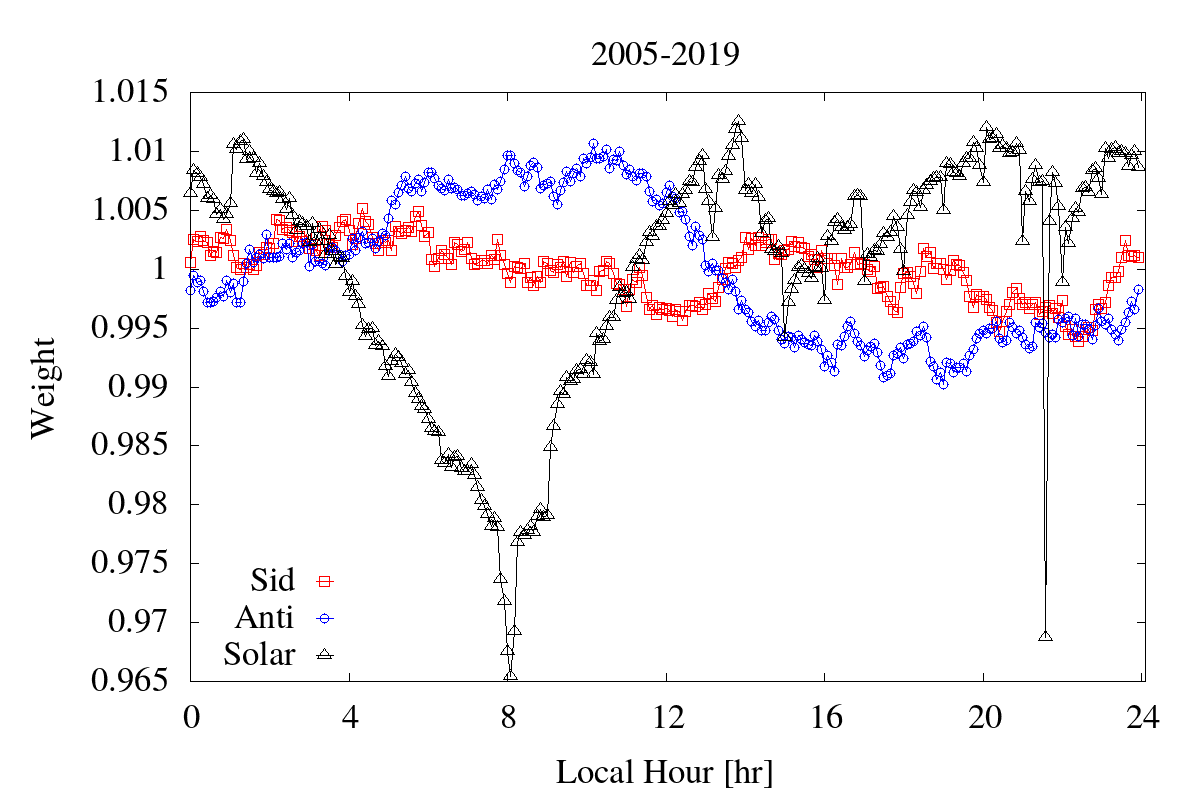
\includegraphics[width=0.85\linewidth]{../report_2_27_04_2020/Graficos/weigth2005-2019.png}
              \caption{Pesos de los hexágonos en el rango 2005-2019 para distintas frecuencias.}
              \label{fig:pesos_ejemplo}
        \end{figure}

  \subsubsection{Cálculo de Rayleigh para una frecuencia dada}

            \begin{enumerate}
        \item Fijando un rango de tiempo, estudiamos una frecuencia en particular, para el cálculo consideramos el periodo $T$
        \item Con los eventos ya filtrados, clasifico cada evento $i$ según la hora local por un fase
        \begin{equation*}
          h = (\text{hora local del evento } i)\times \frac{T}{T_{Solar}}
        \end{equation*}
        \item Este paso es parecido al paso $3$ del peso de los hexágonos donde obtengo $h'$ a partir de $h$. A diferencia que en este proceso, no es importante la cantidad de hexágonos, sino los pesos asignados a cada segmento en  la sección \ref{peso_hexagonos}. Una vez que le asigno un segmento $k$ a un evento $i$, el mismo pasa a tener un peso dado por:
        \begin{equation*}
          \text{peso del evento } i = w_{i}= (w_{k, hex})^{-1}
          \end{equation*} 
         
        \item Para el análisis en frecuencias, se necesita calcular los coeficientes de Fourier del primer armónico $a$ y $b$, para este caso se calculan de la siguiente manera:

        \begin{enumerate}
          \item Por cada evento se calculan los siguientes valores:
          \begin{align}
             a_i' &= {w_i}\cos\Big(2\pi \frac{h'}{24} + RA_i -RA_{cenit,i}\Big)\\
             b_i' &= {w_i}\sin\Big(2\pi \frac{h'}{24} + RA_i -RA_{cenit,i}\Big)\\
         \end{align}
         
         \item Una vez que se obtuvieron los valores de $a_i'$ y $b_i'$ para todos los eventos en el rango de tiempo estudiado, se calculan los coeficientes mediante:
         \begin{alignat}{1}
          \mathcal{N} &= \sum^{Eventos}_i w_i\\ 
            a &= \frac{2}{\mathcal{N}} \sum^{Eventos}_i a_i' \qquad
            b = \frac{2}{\mathcal{N}} \sum^{Eventos}_i b_i'  
         \end{alignat}
        \end{enumerate}

        \item Con los coeficientes es posible calcular la amplitud de la frecuencia estudiada $\tilde{r}$ y la fase $\phi$. Otros parámetros calculados para el análisis son la probabilidad $P(\tilde{r})$ de que la amplitud obtenida sea producto de una variación de ruido, y el valor de amplitud $r_{99}$ para que dicha probabilidad sea del $1$\%. 
        \begin{alignat}{3}
            \tilde{r} &= \sqrt{a^2 +b^2}             
            &&\phi&&= \arctan\frac{a}{b}\\
            P(\tilde{r})&= \exp(-\mathcal{N}\frac{\tilde{r}^2}{4}) \qquad
            &&r_{99}&&= \sqrt{\frac{-4\log(0.01)}{\mathcal{N}}}
        \end{alignat}



      \end{enumerate}